%\documentclass[final,leqno,onefignum,onetabnum]{siamltexmm}
\documentclass[]{article}
\usepackage{amsmath}
\usepackage{paralist}

\usepackage{graphicx} % Allows including images

\title{Project proposal: Grasp-and-Lift EEG Detection\thanks{From a Kaggle competition}} 

\author{Anirudhan J Rajagopalan, Michele Cer\'u\thanks{New York University (\email{ajr619@nyu.edu}; \email{mc3784@nyu.edu}). Questions, comments, or corrections
to this document may be directed to this email address.}}

\begin{document}
\maketitle
\newcommand{\slugmaster}{%
\slugger{siads}{xxxx}{xx}{x}{x---x}}%slugger should be set to juq, siads, sifin, or siims

\begin{abstract}
  This project aims to classify a human's hand motions from his EEG signal data.  This will help in developing Brain-Computer Interface prosthetic devices for restoring a patient's ability to perform basic daily tasks.
  We are provided with time series EEG recordings of the subjects performing the hand actions which we wish to identify.
  The baseline implemenation uses Convolutional Neural Networks for classifying the hand motion.  The baseline model has an accuracy of 0.98109 MCAUC\@.  
  We propose to apply Fast Fourier Transformation on the signals to generate vectors of frequencies and then use the Fisher Vector\cite{fisher} to obtain a set of features. 
  With these features we will use Logistic regression with Stohastic Gradient Descent for detecting the hand motions.
  % with a performance greater than or equal to the baseline.
\end{abstract}

\pagestyle{myheadings}
\thispagestyle{plain}
\markboth{Grasp-and-Lift EEG Detection}{Grasp-and-Lift EEG Detection}

\section{Introduction}
%motivation (real-world application, social good, etc.)
The main goal of this project is to identify hand motions from scalp Electroencephalogram (EEG) recordings, as described in the Kaggle competition\cite{kaggle}.
The dataset consists of 3,936 Grasp and Lift (GAL) series, meaning that the analysed subject grasped an object, held it for some seconds and then replaced it (as explained in detail in\cite{experiment}). 
Every time, without acknowledging the subject, two main properties of the object were changed: the  weight, that could be 165g, 330g or 660g, and the contact surface, that could be sandpaper, suede or silk.  In this context there are six events that represents different stages of the hand movements that we aim to predict thorough EEG analysis: 
\begin{enumerate} 
  \item \textit{HandStart}: the beginning of the movement.
  \item \textit{FirstDigitTouch}: making contact with the object.  
  \item \textit{BothStartLoadPhase}: starting to load the object. 
  \item \textit{LiftOff}: holding the object up.
  \item \textit{Replace}: replacing the object in its original position.
  \item \textit{BothReleased}: releasing the fingers from the object. 
\end{enumerate}
The training dataset contains the exact moment when this events occurred during the GAL, that were measured using the 3D position of both hand and object, electromyography signal (EMG) coming form the arm and the hand muscles of the subject, and the force/torque applied to the object. 
An important restriction to take in account while trying to predict this event, is that for a GAL we can use only data collected in past series and not use the futures one.  
This restriction is due to the fact that in a real world application there would be no access to future data.

The study aims to find a correlation between the GAL and the EEG  that could be applied on developing techniques for the control of prosthetic devices. More in general EEG lay at the base of non invasive brain computer interface BCI\cite{BCI}, that doesn't depends on neuromuscular control and therefore could be used to help patient with heavy neuromuscular disorder to interact with the environment (such as patient who have lost hand function). 

\section{Performance Criterion}
We will use Mean Column-wise Area Under the Curve (MCAUC) for evaluating the performance of our output.  That is the mean of individual areas under the ROC curve for each predicted columns.

\section{Problem Formulation}
The training set consists of time series information for twelve subjects performing 30 series of GAL tasks.  We are provided with a data file consisting of the EEG recordings from the 32 electrodes.  The 30 GAL series are split across 8 data files with corresponding events files.

The model we build for learning the data should adher to `No future data' rule\cite{kaggledata} which means that when predicting, we should not use data from the future.  We should also take care not to include data leakage.  For example, we should not center data for a series using the data from future events in the same series.

Each signal is sampled with a 500Hz frequency. We will group the signals in fixed interval of time, each of this temporal window will contain a fixed number of data points $N$, that will be an hyper parameter for the program. Considering the sampling frequency of the data set, the minimum size of the windows will be $0.2 s$ (100 data points inside the temporal window). 
%We will then sample data points in this interval with a frequency $f_s$, that will be another hyper parameter of the program, so the number of sample point considered in the window will be:
%$$
%N=Tf_s
%$$
For each of this window we can then write the Discrete Fourier Transformation (DFT) as:
\begin{equation}
  \label{DFT}
  F(n) =\sum_{k=0}^{N-1}x(k)e^{\frac{2\pi i kn}{N}}
\end{equation}  
Ranging $k$ from $0$ to $N-1$ this equation represent the $N$ frequencies that describe the wave inside the window.\\
Applying the Fast Fourier Transformation (FFT) algorithm\cite{FFT} we will calculate all this frequencies for all windows in the signal. This process will be applied to each of the signals in the data set. The training data set consists of $96$ files with $32$ signals each. Approximately a file has $200,000$ data point, then the total number of data points is $96\times 32 \times 200,000$. If we take windows of $N=100$ number of samples we will have $96\times 32 \times 2,000=6,144,000$ discrete Fourier transformation, and each of them will generate a vector $x_t$. So we will have a set of $X=\{x_t,t=1\dots T\}$ sample vectors. The probability density function  $u_\lambda$  that models this samples
depends on the parameters $[\lambda_1\dots \lambda_M]$ that represent the set of feature that we what to calculate. We will use the Fisher Vector\cite{fisher} to find the features that maximise the log-likelihood:
\begin{equation}\label{loglikelihood}
G_\lambda^X= \nabla_\lambda \log u_\lambda(X)
\end{equation}

%%%%%%%%%%%%%%%%%%%%

%The test set consists of data files for 12 subjects performing GAL\@.
%The input can be represented by a feature vector of size 32 (m = 32).  
%Due to `No future data' rule, we should be careful to center/scale the data only till the series which is being processed at that instant.

Once we have the features, we will then use logistic regression to classify the input events.  We need to use six different classifiers with each corresponding to one of the hand events described in introduction section.  Logistic regression is given by the function
\begin{align*}
  J(\theta) = & \frac{1}{m} \sum_{i = 1}^{m} \mathrm{Cost}(h_{\theta}(x^{i}), y^{(i)}) \\
  = & -\frac{1}{m} [\sum_{i=1}^{m} y^{(i)} \log{h_{\theta}(x^{(i)} )} + (1 - y^{(i)}) \log{( 1 - h_{\theta}(x^{(i)}) )}]
\end{align*}

Where,

h is the sigmoid function of theta.

\(\theta\) is the error funcction

We then minimize \(J(\theta)\) using stochastic gradient descent to find the optimal classifier for the given input set.

\section{Algorithm}
The algorithm used in the baseline consists of two main approaches. The first one applies Logistic Regression and Linear Discriminant Analysis (LDA) on features describing the sample of the dataset. The second one uses Neural Network in a not event-specific way. Convolutional Neural Network is trained to find the correlation between all electrode at equal time (2D spatial correlation) and the correlation between a current event with a set of samples from the past events (1D temporal correlation). Recurrent Neural Network is also used to find temporal correlation.


\section{Baseline method, algorithm, software}
We consider the scripts with most accurate results in the Kaggle competition for baseline\cite{kaggleleaderboard}.  We use the first level implementation by \textit{Cat \& Dog}\cite{kagglewinners} as our baseline.
The baseline method uses Logistic regression with LDA for providing an event specific view of the data.  There were also two level-1 Neural Network approaches that were not event specific.
A small Recurrent Neural Networks trained on lowpass filtered signal and a small Convolutional Neural Network that is trained on a current sample and a subsampled portion of past samples.

We attempted to run the baseline software\cite{baselineSoftware} in a commodity ubuntu virtual machine.  Since the hardware specifications\cite{hardwarespecifications} are far far higher than that available to us right now, we had to find out innovative ways to get the baseline running.

\begin{itemize}
  \item In our first attempt, We tried installing all the dependencies mentioned in an Ubuntu virtual machine and started the level1 scripts.  The scripts ran for more than 8 hours before getting killed due to exceptions.
  \item We figured out that it is better to run the script in a system with more compute resources.  So we tried running the script in NYU HPC clusters.  But due to incompatibility of the required softwares we were unable to get the code running there too even after multiple attempts.  The sample job is available in github link\cite{hpcjob}.
  \item The third option was to create a local VM and run the script on a subset of the original samples.  We figured out that there can be two strategies for getting the sub samples.  
    \begin{inparaenum}[\itshape a\upshape)]
      \item Run the script on the complete GAL series for a fewer number of subjects.
      \item Run the script on the fewer number of series for a all the subjects.
    \end{inparaenum}
    After trying out the first option, we figured out that running the script on fewer series for all subjects will be faster in the commodity machine that we use.  We trimmed down all the training data and event files to 4000 lines (approximately one series) and ran the baseline.  
\end{itemize}

Unfortunately, inspite of all these attempts spanning over two weeks to get the baseline running, we were unable to run the baseline.  We also seeked the help of the author for getting the baseline running.  The author responded with his suggestions.  We were unable to run the baseline even after implementing the author's suggestions\cite{orurepo}.  The log of last run of the baseline script is also uploaded for reference\cite{runlog}.

\section{Short description of the dataset}
The  datasets consist of data collected with 12 subjects, each consisting of approximately 30 grasp and Lift performed. The Data is divided in a training set, containing the first 8 series for each subject, and  the testing set contains the last two series.
In the dataset each of this event correspond to a binary variable (1 if the event is present and 0 otherwise), and we see that the list of event always present in the same other, but the event are not all mutually exclusive meaning that some of  them could be 1 at the same time.  

\section{Preprocessing}
In order to prepare the data for the classification problem, we used the preprocessing EEG library MNE\cite{MNE} that allowed us to load all the potential signals for all the electrodes and deal with them in a compact and cohesive way. The code is uploaded in the github repository\cite{Preprocessing}.\\
 We converted the data into our training set (eight files) to MNE format. For cross validation we take the series from $1$ to $6$ as the training set and the series $7$ and $8$ as validation set.\\  
We loaded the data into a RawArray\cite{MNE} that we used to:
\begin{itemize}
\item Extract epoch information from the RawArray (using a window of 500 samples), that will be used in future to find event related potential ERP.  
\item Find the covariance matrix (of dimension $32\times32$) between all the features for the complete series (splitted in training and validation). 
\end{itemize}
The extracted epoch value are  three dimensional array ($n_s$, $32$,$500$) where $n_s$ are the number of epoch present in the input files. \\
We then used the XDawn filter\cite{MNE} to transform the epoch value according to the covariance matrix.\\
The generated epoch value and the labels are saved in separated files (one for the training set and one for the validation set) as following:\\
epoch value:\\
\url{data/processed/subj{0}_train_data.npy }\\
\url{data/processed/subj{0}_val_data.npy}\\
labels: \\
\url{data/processed/subj{0}_train_labels.npy}\\
\url{data/processed/subj{0}_val_labels.npy}\\
This are the file that we will use further in the pipeline to learn the model.



\section{Pipeline}
\fbox{\parbox[t]{6em}{Preprocessing:\\MNE\\XDawn}}%
\raisebox{-4ex}{$\to$}%
\fbox{\parbox[t]{6em}{Vocabulary learning: \\Bag of words\\VLAD}}%
\raisebox{-4ex}{$\to$}%
\fbox{\parbox[t]{6em}{Dimension reduction:\\ PCA\\ variance$=0.9$}}
\raisebox{-4ex}{$\to$}%
\fbox{\parbox[t]{6em}{ Prediction\\SVM linear and gaussian\\Parameter C\\parameter $ \gamma$}}
\\
Description of all step in the pipeline


\begin{center}
\begin{figure}\caption{AUC result for only one subject run in local. With $k=10^8$ and $C=2^{-4}$ Score$=0.3627$}
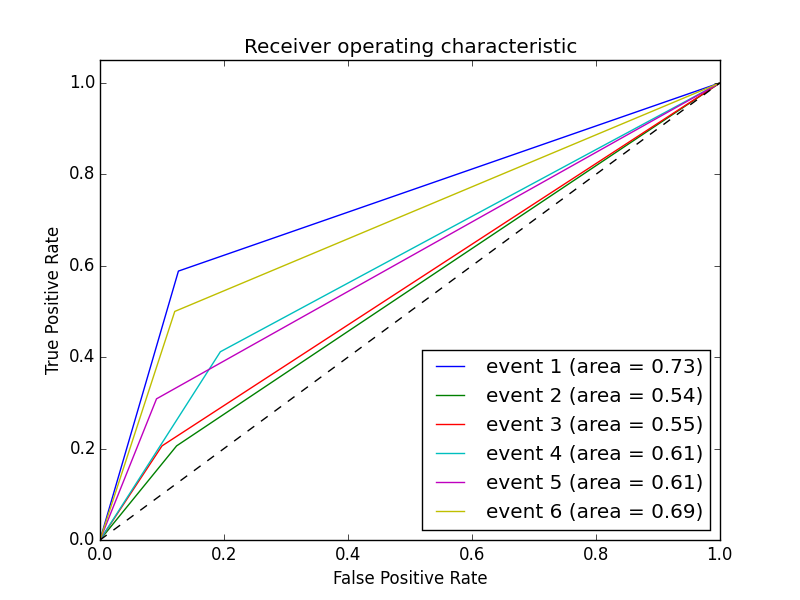
\includegraphics[height=3.0in]{plots/oneSubjectAUC.png}
\end{figure}
\end{center}



\begin{center}
\begin{figure}\caption{AUC result for only one subject run in local. With $k=10^8$ and $C=2^{4}$ Score$=0.5049$}
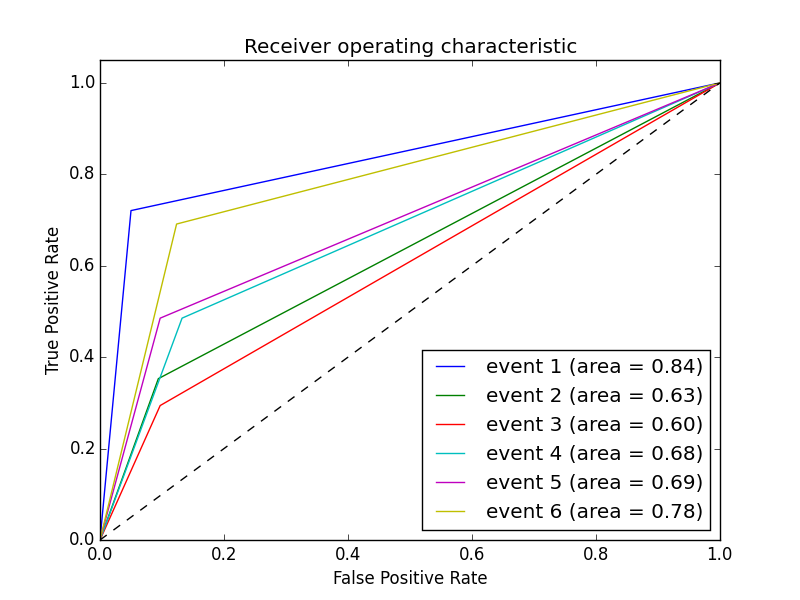
\includegraphics[height=3.0in]{plots/oneSubjectAUCC16.png}
\end{figure}
\end{center}





\section{implementation of Kmeans}

\section{Implementation of VLAD}

\section{Implementation of Bag of words}
Results of bag of words

\section{Grid search}

\begin{table}[]\label{2compTable}
\centering
\caption{Bag of words score for n component$=2$}
\label{2comp}
\begin{tabular}{lllll}
  C      &    K &    score &       time \\                                                                            
0.0625  &  256 & 0.293837 &  20.033333  \\                                                                            
0.1250  &  256 & 0.294705 &  20.833333  \\                                                                            
0.2500  &  256 & 0.295066 &  20.766667  \\                                                                            
0.5000  &  256 & 0.295066 &  22.033333  \\                                                                            
1.0000  &  256 & 0.290075 &  22.566667  \\                                                                            
2.0000  &  256 & 0.290003 &  22.700000  \\                                                                            
4.0000  &  256 & 0.290003 &  28.800000  \\                                                                            
8.0000  &  256 & 0.295573 &  46.966667  \\                                                                            
16.0000 &  256 & 0.289858 &  74.733333  \\                                                                            
0.0625  &  512 & 0.315900 &  26.300000  \\                                                                            
0.1250  &  512 & 0.320529 &  25.000000  \\                                                                            
0.2500  &  512 & 0.330946 &  27.500000  \\                                                                            
0.5000  &  512 & 0.318721 &  30.500000  \\                                                                            
1.0000  &  512 & 0.325882 &  39.166667  \\                                                                            
2.0000  &  512 & 0.326317 &  47.633333  \\                                                                            
4.0000  &  512 & 0.334852 &  67.300000  \\                                                                            
8.0000  &  512 & 0.330729 & 141.166667  \\                                                                            
16.0000 &  512 & 0.322627 & 209.766667  \\                                                                            
25.0000 &  512 & 0.318468 &  26.950000  \\                                                                            
0.0625  & 1024 & 0.352575 &  32.400000  \\                                                                            
0.1250  & 1024 & 0.352213 &  37.566667  \\                                                                            
0.2500  & 1024 & 0.352792 &  39.133333  \\                                                                            
0.5000  & 1024 & 0.358941 &  49.066667  \\                                                                            
1.0000  & 1024 & 0.360749 &  69.033333  \\                                                                            
2.0000  & 1024 & 0.365668 &  79.533333  \\                                                                            
4.0000  & 1024 & 0.369864 & 141.333333  \\                                                                            
8.0000  & 1024 & 0.359520 & 344.700000  \\                                                                            
16.0000 & 1024 & 0.358941 & 475.833333  \\                                                                            
0.0625  & 2048 & 0.430555 &  48.066667  \\                                                                            
0.1250  & 2048 & 0.442564 &  67.966667  \\                                                                            
0.2500  & 2048 & 0.461661 &  59.866667  \\                                                                            
0.5000  & 2048 & 0.474392 &  84.800000  \\                                                                            
1.0000  & 2048 & 0.491392 &  95.733333  \\                                                                            
2.0000  & 2048 & 0.501374 & 132.000000  \\                                                                            
4.0000  & 2048 & 0.516204 & 173.500000  \\                                                                            
8.0000  & 2048 & 0.530237 & 196.500000  \\                                                                            
16.0000 & 2048 & 0.531901 & 317.500000                                                                         
\end{tabular}
\end{table}



From the table (\ref{2compTable}) and the plot (\ref{2compPlot}) we see that the best score is achieved for the maximum value of $C$ and $k$.
 
\begin{center}
\begin{figure}\caption{Time consumed for grid search in the pipeline with number of component=2}\label{time2Components.png}
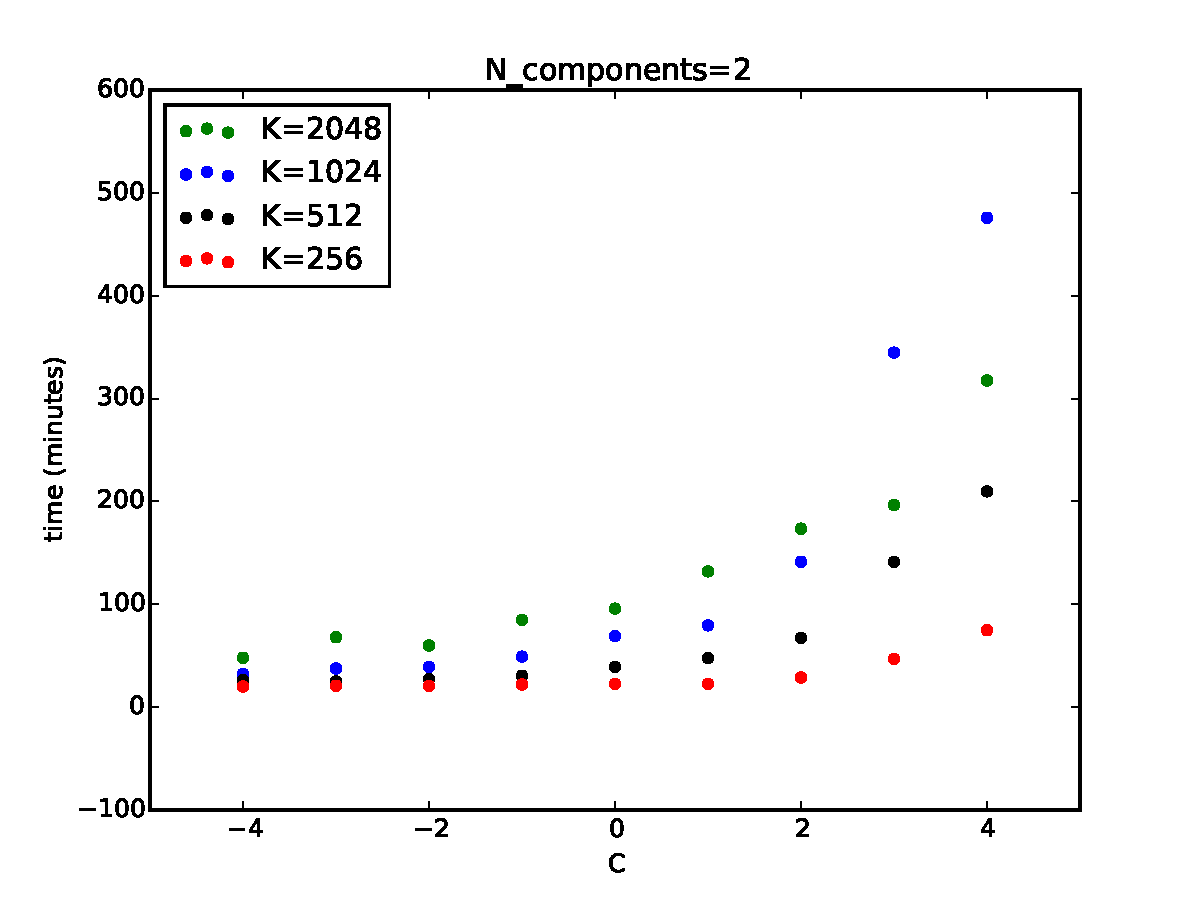
\includegraphics[height=3.0in]{plots/time2Components.pdf}
\end{figure}
\end{center}

\begin{center}\label{2compPlot}
\begin{figure}\caption{Score for grid search in the pipeline with number of component=2}\label{score2Components.png}
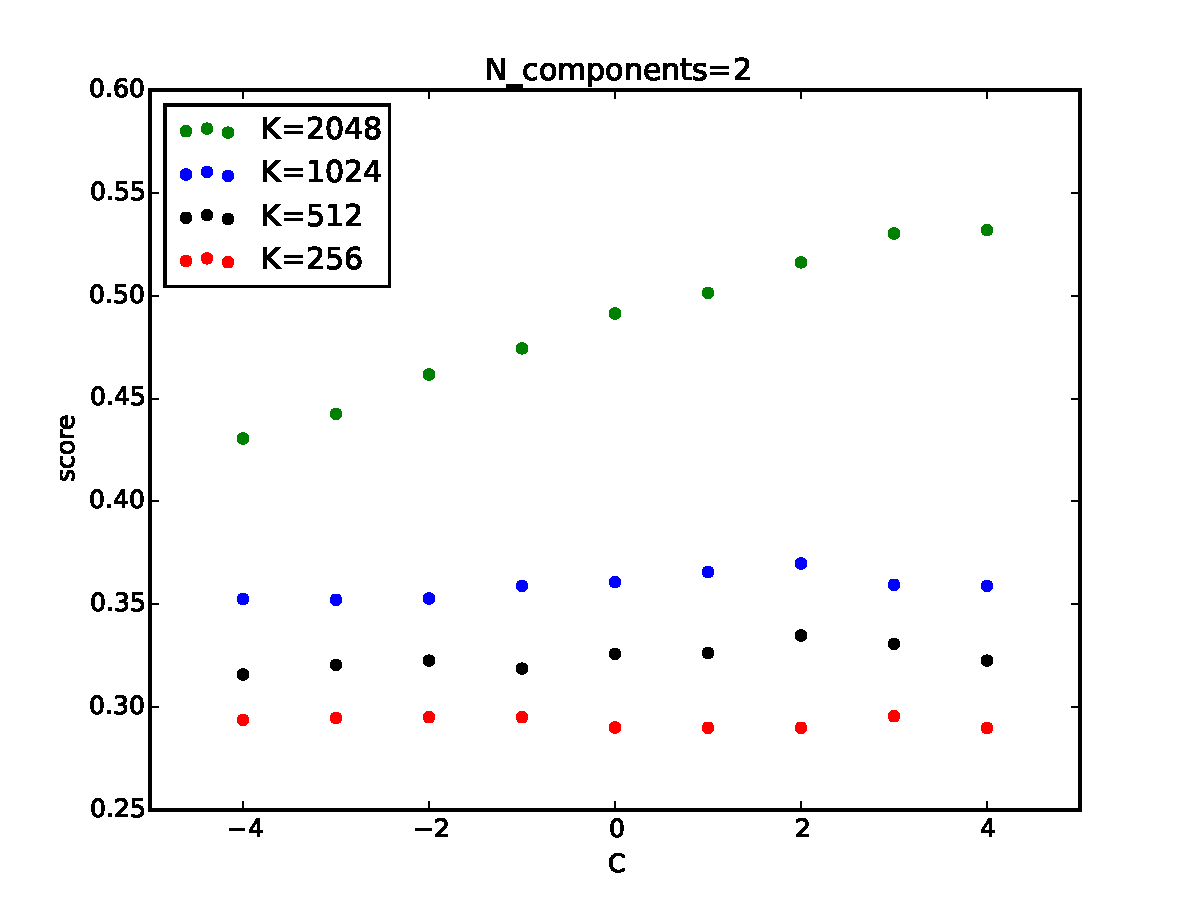
\includegraphics[height=3.0in]{plots/score2Components.pdf}
\end{figure}
\end{center}

in figure \ref{time2Components.png}.











\newpage




%We loaded all the data for the training set and stored it in a MNE Raw object.  We divided the signal into a set of $500$ fix-length epochs that are correlated to the event that we want to detect (HandStart, FirstDigitTouch etc.). 

\begin{thebibliography}{1}
  \bibitem{kaggle} Kaggle competition:  \url{https://www.kaggle.com/c/grasp-and-lift-eeg-detection}
  \bibitem{experiment} \url{http://www.nature.com/articles/sdata201447}
  \bibitem{BCI}D. J. McFarland and J. R. Wolpaw. Brain-computer interfaces for communication and control. Commun. ACM, 54(5):60?66, May 2011.
  \bibitem{baseline}\url{https://github.com/alexandrebarachant/Grasp-and-lift-EEG-challenge}
  \bibitem{model}\url{https://hal.inria.fr/hal-00830491/file/journal.pdf}
  \bibitem{kagglewinners}\url{https://github.com/alexandrebarachant/Grasp-and-lift-EEG-challenge}
  \bibitem{kaggleleaderboard}\url{https://www.kaggle.com/c/grasp-and-lift-eeg-detection/leaderboard}
  \bibitem{kaggledata}\url{https://www.kaggle.com/c/grasp-and-lift-eeg-detection/data}
  \bibitem{fisher}\url{https://hal.inria.fr/hal-00830491/file/journal.pdf}
  \bibitem{FFT}Fast Fourier Transforms, Connexions online book edited by C. Sidney Burrus, with chapters by C. Sidney Burrus, Ivan Selesnick, Markus Pueschel, Matteo Frigo, and Steven G. Johnson (2008)
  \bibitem{baselineSoftware} \url{https://github.com/alexandrebarachant/Grasp-and-lift-EEG-challenge/tree/master/lvl1}
  \bibitem{hardwarespecifications} \url{https://github.com/alexandrebarachant/Grasp-and-lift-EEG-challenge\#hardware}
  \bibitem{hpcjob} \url{https://raw.githubusercontent.com/mc3784/Computational-Machine-Learning-/master/baseline/level1.q}
  \bibitem{orurepo} \url{https://github.com/rajegannathan/grasp-lift-eeg-cat-dog-solution-updated}
  \bibitem{runlog} \url{https://github.com/rajegannathan/grasp-lift-eeg-cat-dog-solution-updated/blob/master/lvl1/typescript}
  \bibitem{MNE}\url{http://mne-tools.github.io/mne-python-intro/}
  \bibitem{Preprocessing}\url{https://github.com/rajegannathan/grasp-lift-eeg-detection}
\end{thebibliography} 


\end{document}
%% end of file `docultexmm.tex'
